\chapter{Survival analysis}

\section{Survival data}
Survival analysis is the field of studying lifetime and time-to-event data. An overview of modelling survival data is \citet{ABG}. We look at a stochastic variable $T>0$ which is the time to some event. To observe such data in real life, we must wait until the event actually happens. This might in some cases never happen, or it might take a very long time. One example is a clinical trial of $n$ patients who have been treated for some disease, and where $T_i$, $i=1,\ldots,n$, is the time until they relapse. Typically these trials are for a set amount of time, say, until $\tau$. Luckily, not every patient relapses during that time, and so their time of relapse $T_i$ is not observed. We could throw away these observations, but we at least know that they survived until $t=\tau$. We therefore work with the concept of incomplete data, which we call \textit{censored} data. An observed lifetime $\tT$ is censored if the actual lifetime $T$ is larger than $\tT$. We can say that we have a censoring mechanism which works such that the observed $\tT=\min(T, C)$, where $C$ is a censoring time. In the clinical trial example mentioned, $C=\tau$. We also need a censoring indicator, $D=I(\tT=T)$, indicating if we have observed the actual event.

\subsection{The survival function $S(t)$}
In survival analysis, one of the things we are interested in is the survival function. The survival function $S(t)$ is the probability of surviving until time $t$,
\begin{align*}
    S(t)=\Pr(T>t)=1-\Pr(T<t)=1-F(t).
\end{align*}
Here $F(t)$ is the familiar cumulative distribution function. If the derivative $f(t)$ of $F(t)$ exists, the lifetime $T$ has probability distribution function $f(t)$.

\subsection{The hazard function $\hz(t)$}
We are also interested in the hazard function. This is the probability of the event happening in a given small interval at time $t$, conditioned on the event not having happened yet. More formally, the hazard function is defined as a limit of this probability as the size of the interval goes to zero,
\begin{equation*}
    \hz(t)=\lim_{\epsilon\to0}\frac{\Pr(T<t+\epsilon|T>t)}{\epsilon}.
\end{equation*}
The hazard function $\hz(t)$ is then the chance of the event happening at time $t$, if it has not happened yet. Estimation of the hazard function is hard, and we do not achieve the usual $\sqrt{n}$ convergence.

Note that
\begin{equation*}
    \Pr(T<t+\epsilon|T>t)=\frac{\Pr(T<t+\epsilon,T>t)}{\Pr(T>t)}=\frac{F(t+\epsilon)-F(t)}{S(t)},
\end{equation*}
and inserting this into the hazard rate yields
\begin{equation}
\label{eq:hfs}
    \hz(t)=\frac{1}{S(t)}\lim_{\epsilon\to0}\frac{F(t+\epsilon)-F(t)}{\epsilon}=\frac{f(t)}{S(t)}=\frac{-S^\prime(t)}{S(t)},
\end{equation}
where the probability distribution function $f(t)$ is obtained by its limit definition, and we note that $S^\prime(t)$ is the derivative of $1-F(t)$, which is $-f(t)$. By integrating the hazard from 0 to time $t$, we get the cumulative hazard function $A(t)=\int_0^t\hz(s)\d s$,
\begin{equation}\label{eq:cumulative-hazard}
    A(t)=-\int_0^t\frac{S^\prime(s)}{S(s)}\d s=-\int_0^t\frac{\frac{\d S}{\d f}}{S(s)}\d s=-\int_0^t\frac{1}{S(s)}\d s=-\log(S(t)).
\end{equation}
Given censored survival data $(t_i,d_i),i=1,\ldots,n$, we introduce the at-risk function $Y(t)$, which is equal to the number of individuals still at risk at time $t$,
\begin{equation*}
    Y(t)=\#\{t\colon t_i\geq t\},
\end{equation*}
where $\#(\cdot)$ is the counting operator over a set. We may then estimate the survival function $S(t)$ by the Kaplan-Meier estimator
\begin{equation*}
    \hat{S}(t)=\prod_{t_i\leq t}1-\frac{d_i}{Y(t_i)},
\end{equation*}
and the cumulative hazard function $A(t)$ by the Nelson-Aalen estimator
\begin{equation*}
    \hat{A}(t)=\sum_{t_i\leq t}\frac{d_i}{Y(t_i)}.
\end{equation*}

\section{Survival data likelihood regression setup}
Given survival data with covariates, $(t_i,d_i,\x_i)$, and parameterized functions $S(t|\x_i,\bbeta)$ and $f(t|\x_i,\bbeta)$ corresponding to a survival distribution, where $\bbeta=(\beta_1,\ldots,\beta_p)$ is a regression coefficient, we want to set up a likelihood for the data. We assume that the data is independent and identically distributed. If the event has occurred, the indicator $d_i$ is 1. We can then use the information about the lifetime distribution, such that the single individual $i$ contributes
\begin{equation}\label{eq:f}
    f(t_i|\xi)
\end{equation}
to the likelihood. If the event has not occurred, the observation is censored, and $d_i$ is 0. In this case, we do not have the actual lifetime, and so we cannot use the lifetime distribution, but we must rather use the survival distribution. Therefore this observation contributes
\begin{equation}\label{eq:S}
    S(t_i|\xi)
\end{equation}
to the likelihood. Of course, since an observation can only be either censored or not censored at the same time, $\di$ is either 0 or 1. If the event has occurred, $d_i$ is 1, and then $1-d_i$ is 0. Similarly, if the event has not occurred and the event is censored, then $d_i$
 is 0, and then $1-d_i$ is 1. This allows us to take the product of \eqref{eq:f} and \eqref{eq:S} where we take these to the power of $\di$ and $1-\di$, respectively, so that a single observation contributes
\begin{equation*}
    f(\ti|\x_i)^{\di}S(\ti|\x_i)^{1-\di}
\end{equation*}
to the likelihood. Since we assume the observations to be independent, the likelihood of the observed sample as a whole is the product of the single likelihoods. The complete likelihood becomes
\begin{equation}\label{eq:surv-lik}
    L(\bbeta)=\prod_{i=1}^n f(t_i|\x_i,\bbeta)^{d_i} S(t_i|\x_i,\bbeta)^{1-d_i}.
\end{equation}
Since it is more convenient to work with the log likelihood, we calculate this as well,
\begin{align}\label{eq:surv-lik}
\begin{split}
    l(\bbeta)&=\log L(\bbeta) \\
    &=\sum_{i=1}^n\left[ d_i \log f(t_i|\x_i,\bbeta) + (1-d_i)\log S(t_i|\x_i,\bbeta)\right].
\end{split}
\end{align}
Note that since $\log S(t)=-A(t)$ \eqref{eq:cumulative-hazard} and $f(t)=\alpha(t)S(t)$ \eqref{eq:hfs}, this further simplifies to
\begin{equation*}
    l(\bbeta)=\sum_{i=1}^n\left[ d_i \log \hz(t_i|\x_i,\bbeta) - A(t_i|\x_i,\bbeta)\right].
\end{equation*}

\section{Proportional hazards regression}
So far we have not introduced covariates. How may we use a covariate vector $\x$ in modelling, say, the hazard rate? A very common model to choose here is that of a proportional hazards model,
\begin{equation}\label{PH}
    \hz(t|\x)=\hz_0(t)r(\x|\bbeta),
\end{equation}
where $\hz_0(t)$ is an \textit{unspecified} baseline hazard function shared between all individuals, and $r(\x|\beta)$ is a so-called relative risk function parameterized with regression coefficient $\bbeta=(\beta_1,\ldots,\beta_p)$. We choose $r(\x)$ such that it is appropriately normalized, meaning $r(\0)=1$. A vital assumption here is that the covariates are fixed in time. With this setup, it turns out that we can do regression without specifying the baseline hazard. This is a major advantage, because we then do not have to think about modelling effects in time. Given data $(t_i,d_i),i=1,\ldots,n$, we may set up a so-called partial likelihood.  For all observations $i=1,\ldots,n$ with $d_i=1$, we know that there is an event at time $t_i$. The probability of the event happening for some individual $j$ is the hazard, i.e., the instantaneous probability of that individual at that time, divided by the sum of all such hazards for those individuals still alive. Assuming that observations are independent and identically distributed, the partial likelihood for the data is then the product of all such ratios,
\begin{equation*}
    \pl(\bbeta)=\prod_{d_i=1}\frac{\Pr(\text{event happens to }i\text{ at time }t_i)}{\sum_{j\in R(t_i)}\Pr(\text{event happens to }j\text{ at time }t_i)}=\prod_{d_i=1}\frac{\hz_0(t_i)r(\x_i)}{\sum_j \hz_0(t_i)r(\x_j)},
\end{equation*}
where we see that the baseline hazard will cancel out, and we are left with just the relative risk functions.

The most common choice, by far, for $r(\x)$ is the Cox model \citep{cox},
\begin{equation*}
    r(\x)=\exp(\x^T\bbeta).
\end{equation*}
This is an attractive model because the effect of a unit increase in an element of $\bbeta$ has a nice interpretation. Assume we have two covariates $\x_1$ and $\x_2$, and that $\x_2$ is equal to $\x_1$ except for in element $j$, where $x_{2j}=x_{1j}+1$. Then the ratio of the two hazard rates becomes
\begin{equation*}
    \frac{\exp(\x_2^T\bbeta)}{\exp(\x_1^T\bbeta)}=\exp((\x_2-\x_1)^T\bbeta)=\exp(\beta_j).
\end{equation*}
Cox regression is used very much in applied research.

\todo[inline]{add Cox regression example}

%\subsection{Cox regression example}
%Lorem ipsum.

\subsection{The proportional hazards assumption}
When we say \eqref{PH}, that $\hz(t|\x)=\hz_0(t)r(x|\bbeta)$, we make the proportional hazards (PH) assumption: We assume that the ratio between the hazard function of two individuals is the same \textit{at all times}. This is a very large assumption to make, and in practice, it is very often not the case. One way to test this assumption for a covariate $j=1,\ldots,p$, is to fit a model $r(x_j)=\exp(f(x_j))$, where $f(\cdot)$ is some spline regression function, and plot it against $x_j$.

\subsection{Robustness of Cox when the PH assumption is violated}
Although the PH assumption is often not valid, in practice, Cox regression tends to work well. \todo[inline]{Need to find a citation here.}

\section{First hitting time models or threshold regression}
So far we have not thought much about how a time-to-event is generated. Instead, we have modelled the hazard rate directly. We have simply said that we have stochastic lifetimes. At one time, an individual is alive, and at a slightly later time, it is perhaps dead. One way to think about how these times are generated is to imagine that each individual has an underlying stochastic process, a health process $Y(t)$, say. Since the process is a function of time, it has a non-negative domain, $t\geq0$. This health process is not observable, but when it hits a certain boundary set $\mathcal{B}$, the individual dies. $\mathcal{B}$ is also called a barrier or a threshold, depending on what kind of set it is, and what association one wishes to envoke. The lifetime $T$, then, becomes the time it takes for the health process $Y(t)$ to enter the boundary set $\mathcal{B}$. In general, the health process $Y(t)$ takes values in a set $\mathcal{Y}$, with an initial value $y_0=Y(0)$. The barrier is a subset of this set of values, $\mathcal{B}\in\mathcal{Y}$, with the initial health process value $y_0\notin\mathcal{B}$. In other words, the lifetime is
\begin{equation*}
    T=\argmin_{t}Y(t)\in\mathcal{B}.
\end{equation*}
First hitting time (FHT) models were introduced in \citet{whitmore1986}, and a good reference paper on the topic is \citet{leewhitmore2006}. Note that these authors use the term threshold regression. We have, together with \citet{caroni2017}, chosen to not use this term, as it is also the name of an already established, and quite different, field of econometrics. FHT models have been applied to many different fields, including medicine, engineering, and economics. They may describe the survival time of a transplant patient, the duration time of a strike, the failure time of an engineering system, and so on.

The first hitting time model framework is highly flexible. We have flexibility both in choice of process, boundary and initial value. The most important part is the stochastic process. Examples include Wiener processes, Markov chains, Bernoulli processes, and Gamma processes. We choose to use the Wiener process, because it has a simple intuition behind it, and it yields a fully parametric regression model.

\subsection{Wiener process}
Let $W(t)$ be a continuous stochastic process defined for $t\in[0,\infty)$, taking values in $\R$, and with initial value $W(0)=0$. If $W$ has increments that are independent and normally distributed with
\begin{equation*}
    \E[W(s+t)-W(t)]=0\text{   and   }\Var[W(s+t)-W(t)]=s,
\end{equation*}
we call $W$ a Wiener process. In other words, each increment has expectation 0 and has standard deviation proportional to the length of the time interval. The position of the process at time $t$ always follows a Gaussian distribution $N(0, t)$ \citep{ABG}. To increase the flexibility of the Wiener process, we can introduce a new process $Y$,
\begin{equation}\label{wiener}
    Y(t)=y_0-\mu t+\sigma W(t),
\end{equation}
which is called a Wiener process with initial value $y_0$, drift coefficient $\mu$, and diffusion coefficient $\sigma$. Introductions to many aspects of Wiener processes are found in \citet{cox1965}. Figure \ref{plot:wiener} shows examples of 5 Wiener process paths with initial value $y_0=10$ and negative drift $\mu=1$.
\begin{figure}[H]
\label{plot:wiener}
\caption{Example of 5 Wiener process paths with initial value $y_0=10$ and negative drift $\mu=1$.}
\centering
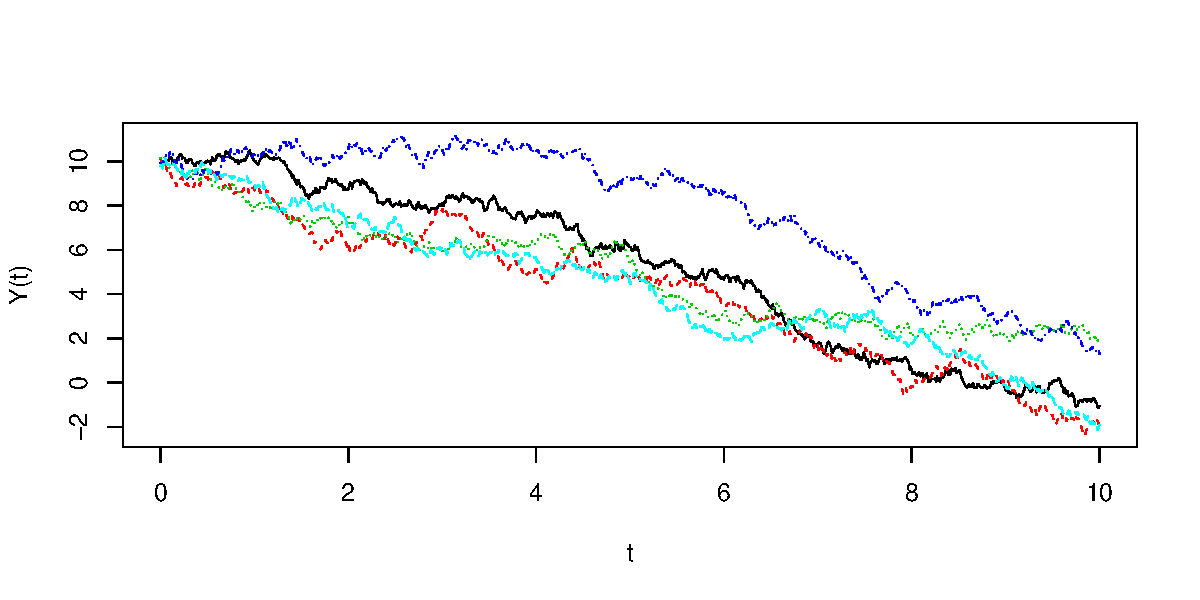
\includegraphics[scale=0.4]{figures/wiener_processes.pdf}
\end{figure}

\subsection{FHT with Wiener process leads to Inverse Gaussian lifetimes}
If we choose the stochastic process to be a Wiener process like in \eqref{wiener}, and we let the boundary be the non-positive numbers, $\setB=(-\infty,0]$, then the lifetime is the time it takes for the process to first reach a non-positive value,
\begin{equation}
    T=\argmin_{t}Y(t)\leq0.
\end{equation}
Note that since the Wiener process is continuous, there will not be a difference between $\leq$ and $<$.

This is a very conceptually appealing model, because it assumes that individuals might have different initial levels, and that also the drift might be different between individuals. It is also attractive because it has closed-form probability and cumulative density functions, and its likelihood is computationally simple. There are no restrictions on the movements of the process, meaning, it is non-monotonic. If we do want a monotonic restriction on the movement of the process, we may use a gamma process \citep{leewhitmore2006}.

It can be shown that the first hitting time of the Wiener process follows an inverse Gaussian distribution \citep{chhikara1988}, with probability distribution function
\begin{equation}
\label{eq:ig-pdf}
    f(t|y_0,\mu,\sigma^2)=\frac{y_0}{\sqrt{2\pi\sigma^2t^3}}\exp\left[-\frac{(y_0+\mu t)^2}{2\sigma^2t}\right],
\end{equation}
and cumulative distribution function
\begin{equation}
\label{eq:ig-cdf}
    F(t|\mu,\sigma^2,y_0)=\Phi\sqb*{-\frac{(\mu t+y_0)}{\sqrt{\sigma^2t}}}+\exp\p*{-\frac{2y_0\mu}{\sigma^2}}\Phi\sqb*{\frac{\mu t-y_0}{\sqrt{\sigma^2t}}}.
\end{equation}
%See Appendix \todo{TO DO!} for the mathematical derivation.
Note that if the drift $\mu$ is positive, then it is not certain that the process will ever reach 0. Hence the probability distribution function in \eqref{eq:ig-pdf} is improper. In this case, the probability of the time not being finite is
\begin{equation*}
    \Pr{}(T=\infty)=1-\Pr{}(T<\infty)=1-\exp{(-2y_0\mu)} \text{ \citep{cox1965}}.
\end{equation*}
Since we in survival analysis prefer working with the survival function $S(t)=1-F(t)$ rather than the cdf $F(t)$, we note that it becomes
\begin{equation}
\label{eq:ig-surv}
    S(t|\mu,\sigma^2,y_0)=\Phi\sqb*{\frac{\mu t+y_0}{\sqrt{\sigma^2t}}}-\exp\p*{-\frac{2y_0\mu}{\sigma^2}}\Phi\sqb*{\frac{\mu t-y_0}{\sqrt{\sigma^2t}}},
\end{equation}
where $\Phi(x)$ is the cumulative distribution function of the standard normal, i.e.,
\begin{equation}
    \Phi(x)=\int_{-\infty}^x\exp\left(\frac{-y^2}{2}\right)/\sqrt{2\pi}\dy,
\end{equation}
and in \eqref{eq:ig-surv} we used the fact that $1-\Phi(-x)=\Phi(x)$, since the standard normal distribution is symmetric around 0.

\subsection{The inverse gaussian is overdetermined if the health process is latent}
There are three parameters in the inverse Gaussian distribution, namely $y_0, \mu$ and $\sigma$. We observe, however, that both the pdf $f(t|y_0,\mu,\sigma^2)$ in \eqref{eq:ig-pdf} and the survival function $S(t|\mu,\sigma^2,y_0)$ in \eqref{eq:ig-surv} only depend on these parameters through $\mu/\sigma$ and $y_0/\sigma$. Hence, there are only two free parameters. In other words, we can without loss of generality fix one parameter, for instance set $\sigma$ equal to 1. This is the conventional way to do it \citep{leewhitmore2006}.

\subsection{The shape of the hazard rate}
The hazard rate is obtained from $\hz(t)=f(t)/S(t)$ \eqref{eq:hfs}. Regardless of initial value, this converges to the same limiting hazard. If $y_0$ is close to zero, we essentially get a decreasing hazard rate. If $y_0$ is far from zero, this gives an essentially increasing hazard rate. If $y_0$ is somewhat inbetween, we get a hazard rate which first increases and then decreases \citep{ABG}.

\todo[inline]{Add plots of hazard rates here.}

\subsection{Comparison of hazard rates}
Of particular interest might be looking at the ratio between two hazard rates, that is, one hazard divided by the other. We might for example look at it when the drift $\mu$ is the same, but the initial level $y_0$ is different. Then the hazard ratio is strongly decreasing. It is also of interest to do the converse, that is, look at the hazard ratio when the initial level is the same, but the drift is different. The result here is quite different. The ratio of the hazards has a ``bathtub'' shape, which levels off at a later time \citep{ABG}. Keep in mind here that levelling off means getting to proportional hazards. The hazard function converges to
\begin{equation}
    \lim_{t\to\infty}\hz(t)=\frac{1}{2}\left(\frac{\mu}{\sigma}\right)^2=0.5\mu^2
\end{equation}
We see that the FHT framework with a Wiener process is a highly flexible parametric model for survival analysis. Indeed, much more flexible than Cox regression, since the hazard ratios in Cox are all confined to be constant over time.

\subsection{Regression}
We may introduce effects from covariates by allowing $\mu$ and $y_0$ to depend on covariates $\x$ and $\z$. A simple and much used model is to simply use the identity link function for the drift $\mu$, and to use the logarithm link function for the initial level $y_0$, since it must be positive in our framework.
\begin{align}\label{eq:coeffs}
\begin{split}
    \mu&=\bbeta^\T\x=\sum_{j=1}^p \beta_jx_j \\
    \ln y_0&=\bgamma^\T\z=\sum_{j=1}^d \gamma_jz_j
\end{split}
\end{align}
Here $\bbeta\in\R^p$ and $\bgamma\in\R^d$ are vectors of regression coefficients. Note that we may let $\x$ and $\z$ share none, some, or all elements. We will discuss consequences of this later.

Inserting the pdf \eqref{eq:ig-pdf} and the survival function \eqref{eq:ig-surv} into the log-likelihood \eqref{eq:surv-lik}, we get that the log-likelihood of a survival data set with the inverse gaussian FHT model is
\begin{align}\label{eq:loglik}
\begin{split}
    l(y_0,\mu,\sigma)=\sum_{i=1}^n&\di\p*{\ln y_0-\frac{1}{2}\ln\p*{2\pi\sigma^2\ti^3}-\frac{\p*{y_0+\mu\ti}^2}{2\sigma^2\ti}} \\
    &+
    (1-\di)\ln\p*{\Phi\p*{\frac{\mu\ti+y_0}{\sqrt{\sigma^2\ti}}}-\exp\p*{-\frac{2y_0\mu}{\sigma^2}}\Phi\p*{\frac{\mu\ti-y_0}{\sqrt{\sigma^2\ti}}}}.
\end{split}
\end{align}

\subsection{Fitting an IG FHT model}
At the moment, the standard for fitting an inverse gaussian FHT model to survival data is to use numerical likelihood maximization \cite{caroni2017}. A few software packages exist for doing this, and one of these for \verb|R| \cite{Rlang} is the \verb|threg| package \cite{threg}. There does not exist any method to fit a \textit{regularized} model at the moment, nor to do automatic variable selection. \textbf{This is the reason for my thesis.}

\todo[inline]{Add regression example}

%\subsection{Example of application}
%Lorem ipsum some example. Just use numerical maximization.

%\subsection{Identification problems}